\item \textbf{{[}IJC/PRELIM/9597/2018/P1/Q4{]} }

Bowling is a sport in which a \textquoteleft bowler\textquoteright{}
rolls a bowling ball down a synthetic lane and towards ten pins positioned
at the end of the lane. The objective is to score points by knocking
down as many pins as possible. 
\begin{center}
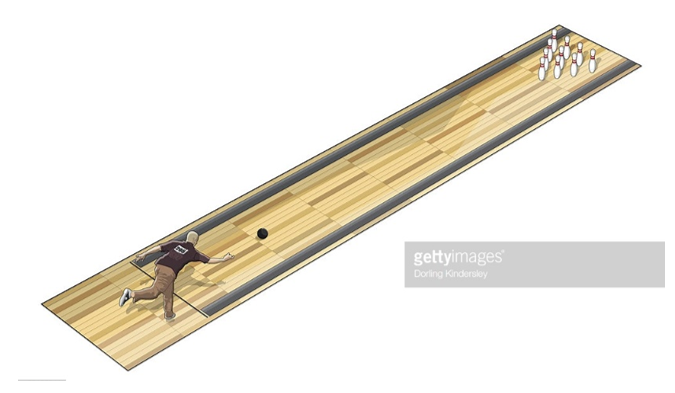
\includegraphics[width=0.5\paperwidth]{C:/Users/Admin/Desktop/Github/question_bank/LyX/static/img/9597-IJC-2018-P1-Q4}
\par\end{center}

\textbf{A bowling game }

One game of bowling consists of ten frames. Each frame consists of
two chances for the bowler to knock down ten pins.

\textbf{Strikes and spares }

Knocking down all ten pins on the first roll of any frame is called
a \textbf{strike}, denoted by \textquoteleft X\textquoteright{} on
the score sheet. If a bowler takes two rolls to knock down all ten
pins, it is called a \textbf{spare}.

\textbf{Scoring and bonus scoring}

Each pin that is knocked down is worth 1 point. 

A strike is worth 10 points plus the number of pins hit on the next
two rolls.

A spare is worth 10 points plus the number of pins hit on the next
roll.

The total score for a game ranges from 0 to 300 points.

\textbf{The tenth frame }

A bowler who strikes or spares the tenth frame will be given one extra
roll. The number of pins hit on this roll will be added to the bowler\textquoteright s
score.

\textbf{Sample Scores} 

\begin{tabular}{|c|c|c|c|c|c|c|c|c|c|c|}
\hline 
Frame & 1 & 2 & 3 & 4 & 5 & 6 & 7 & 8 & 9 & 10\tabularnewline
\hline 
Result & \textbf{\uline{X}} & 7|\textbf{\uline{3}} & 7|2 & 9|\textbf{\uline{1}} & \textbf{\uline{X}} & \textbf{\uline{X}} & \textbf{\uline{X}} & 2|3 & 6|\textbf{\uline{4}} & 7|\textbf{\uline{3}}|3\tabularnewline
\hline 
Frame Score & 20 & 17 & 9 & 20 & 30 & 22 & 15 & 5 & 17 & 13\tabularnewline
\hline 
Cumulative Score & 20 & 37 & 46 & 66 & 96 & 118 & 133 & 138 & 155 & 168\tabularnewline
\hline 
\end{tabular}

\begin{tabular}{|c|c|c|c|c|c|c|c|c|c|c|}
\hline 
Frame & 1 & 2 & 3 & 4 & 5 & 6 & 7 & 8 & 9 & 10\tabularnewline
\hline 
Result & 0|5 & 8|0 & \textbf{\uline{X}} & 0|5 & \textbf{\uline{X}} & 6|\textbf{\uline{4}} & 0|5 & 8|1 & 9|\textbf{\uline{1}} & 5|0\tabularnewline
\hline 
Frame Score & 5 & 8 & 15 & 5 & 20 & 10 & 5 & 9 & 15 & 5\tabularnewline
\hline 
Cumulative Score & 5 & 13 & 28 & 33 & 53 & 63 & 68 & 77 & 92 & 97\tabularnewline
\hline 
\end{tabular}

\begin{tabular}{|c|c|c|c|c|c|c|c|c|c|c|}
\hline 
Frame & 1 & 2 & 3 & 4 & 5 & 6 & 7 & 8 & 9 & 10\tabularnewline
\hline 
Result & \textbf{\uline{X}} & \textbf{\uline{X}} & \textbf{\uline{X}} & \textbf{\uline{X}} & 9|\textbf{\uline{1}} & \textbf{\uline{X}} & 0|0 & 2|2 & 8|\textbf{\uline{2}} & \textbf{\uline{X}}|X|X\tabularnewline
\hline 
Frame Score & 30 & 30 & 29 & 20 & 20 & 10 & 0 & 4 & 20 & 30\tabularnewline
\hline 
Cumulative Score & 30 & 60 & 89 & 109 & 129 & 139 & 139 & 143 & 163 & 193\tabularnewline
\hline 
\end{tabular}

The following algorithms calculate the total score for a bowling game.

\noindent %
\noindent\begin{minipage}[t]{1\columnwidth}%
\texttt{//Used interchangeably in the code for readability}

\texttt{Ten <- 'X'}

\texttt{Strike <- Ten}

\texttt{\bigskip{}
}

\texttt{//Converting the 'X' or 'number' to INTEGER }

\texttt{FUNCTION Pins(Throw as STRING)}

\texttt{\qquad{}IF Throw = Ten THEN}

\texttt{\qquad{}\qquad{}RETURN 10}

\texttt{\qquad{}ELSE}

\texttt{\qquad{}\qquad{}RETURN INTEGER(Throw)}

\texttt{\qquad{}ENDIF }

\texttt{END FUNCTION}

\texttt{\bigskip{}
}

\texttt{//Recursive Procedure }

\texttt{FUNCTION Bowling\_Score(Throws as STRING)}

\texttt{\bigskip{}
}

\texttt{\qquad{}//Helper function to keep track of current frame
number}

\texttt{\qquad{}FUNCTION Bowling\_Score\_Helper(Throws as STRING,
Frame\_Num as INTEGER) }

\texttt{\bigskip{}
}

\texttt{\qquad{}\qquad{}//Frame 10 with no bonus }

\texttt{\qquad{}\qquad{}IF Frame\_Num = 10 AND LENGTH(Throws) =
2 THEN }

\texttt{\qquad{}\qquad{}\qquad{}RETURN SUM(Pins(Throws{[}0{]}),
Pins(Throws{[}1{]})) }

\texttt{\qquad{}\qquad{}ENDIF}

\texttt{\bigskip{}
}

\texttt{\qquad{}\qquad{}//Frame 10 with bonus}

\texttt{\qquad{}\qquad{}IF Frame\_Num = 10 AND LENGTH(Throws) =
3 THEN}

\texttt{\qquad{}\qquad{}\qquad{}RETURN SUM(Pins(Throws{[}0{]}),Pins(Throws{[}1{]}),Pins(Throws{[}2{]})) }

\texttt{\qquad{}\qquad{}ENDIF}

\texttt{\bigskip{}
}

\texttt{\qquad{}\qquad{}//A Strike }

\texttt{\qquad{}\qquad{}IF Throws{[}0{]} = Strike THEN}

\texttt{\qquad{}\qquad{}\qquad{}Frame\_Score <- 10 + SUM(Pins(Throws{[}1{]}),
Pins(Throws{[}2{]}))}

\texttt{\qquad{}\qquad{}\qquad{}RETURN Frame\_Score + Bowling\_Score\_Helper(Throws{[}1:{]},
Frame\_Num + 1) }

\texttt{\qquad{}\qquad{}ENDIF}

\texttt{\bigskip{}
}

\texttt{\qquad{}\qquad{}Frame\_Score <- SUM(Pins(Throws{[}0{]}),
Pins(Throws{[}1{]}))}

\texttt{\bigskip{}
}

\texttt{\qquad{}\qquad{}//A Spare}

\texttt{\qquad{}\qquad{}IF Frame\_Score = 10 THEN}

\texttt{\qquad{}\qquad{}\qquad{}RETURN 10 + Pins(Throws{[}2{]})
+ Bowling\_Score\_Helper(Throws{[}2:{]}, Frame\_Num + 1)}

\texttt{\qquad{}\qquad{}ENDIF}

\texttt{\bigskip{}
}

\texttt{\qquad{}\qquad{}//Frame with no bonus }

\texttt{\qquad{}\qquad{}RETURN Frame\_Score + Bowling\_Score\_Helper(Throws{[}2:{]},
Frame\_Num + 1)}

\texttt{\qquad{}END FUNCTION}

\texttt{\bigskip{}
}

\texttt{\qquad{}RETURN Bowling\_Score\_Helper(Throws, 1) }

\texttt{END FUNCTION }%
\end{minipage}

Note: The above pseudocode is available in the text file \texttt{PSEUDOCODE\_TASK\_4\_1.TX}T
but with \textquoteleft \texttt{=}\textquoteright{} used in place
of \textquoteleft <-\textquoteright{} shown above.

\subsection*{Task 4.1 }

Write a program to calculate a bowling score using the algorithms
provided on the previous page.

\subsection*{Evidence 8 }

Your program code for Task 4.1.\hfill{} {[}5{]}

\subsection*{Evidence 9 }

Screenshot of the results of the following function calls: 
\begin{enumerate}
\item[1.] \texttt{ Bowling\_Score('X2815X91X365452X0X')}\hfill{} {[}1{]}
\item[2.]  \texttt{Bowling\_Score('91739182X90X90X82X')} \hfill{} {[}1{]}
\end{enumerate}

\subsection*{Task 4.2 }

Draw up a list of \texttt{three} suitable test cases. Complete a table
with the following headings: 
\noindent \begin{center}
\begin{tabular}{|c|c|c|}
\hline 
Bowling Score & Purpose of the test & Expected Output \tabularnewline
\hline 
 &  & \tabularnewline
\hline 
 &  & \tabularnewline
\hline 
 &  & \tabularnewline
\hline 
\end{tabular}
\par\end{center}

Amend your program code to include the handling of the test cases
listed in your table. 

\subsection*{Evidence 10 }

The completed table.\hfill{} {[}3{]}

\subsection*{Evidence 11 }

Your amended program code that includes \textbf{internal commentary}.
\hfill{} {[}3{]}

\subsection*{Evidence 12 }

Screenshots for each test data run. {[}3{]}\quad{} 

At the 2018 Singapore Championship, bowlers play a total of six games
each in the qualifying round. The eight bowlers with the highest total
score qualify for the Masters Competition. You may assume that there
are no bowlers with the same total score.

\texttt{SCORES.TXT} is a text file containing the register number,
country and the scores for six games of twenty bowlers in the qualifying
round, with one bowler per line in the format: 
\noindent \begin{center}
\texttt{<Register Number> <Country> <Score 1> <Score 2> \dots{} <Score
6>}
\par\end{center}

For example: 
\noindent \begin{center}
\texttt{157 MAS XXXXX9091XXX82 90XXXXXXXXXX9 \dots{} 8172XXXX919191XX8}
\par\end{center}

\subsection*{Task 4.3 }

Design and write program code to:
\begin{itemize}
\item Read the entire contents of \texttt{SCORES.TXT}. 
\item Calculate the score of each game for all twenty bowlers, using your
code in \textbf{Evidence 8}. You may assume that all the scores in
\texttt{SCORES.TXT} are valid scores.
\item Calculate the total score for each bowler and store this in an appropriate
data structure together with the respective \texttt{Register Number}
and \texttt{Country}. 
\item Use \textbf{bubble sort} to sort the bowlers according to their total
score. 
\item Output the Official Results of the competition.
\end{itemize}
An example of the output should look like this:
\noindent \begin{center}
\begin{tabular}{cccc}
\multicolumn{4}{c}{\texttt{Official Results}}\tabularnewline
\texttt{Position} & \texttt{Register Number} & \texttt{Country} & \texttt{Total Score}\tabularnewline
\texttt{1} & \texttt{175} & \texttt{SIN} & \texttt{1734}\tabularnewline
\texttt{2} & \texttt{299} & \texttt{SIN} & \texttt{1724}\tabularnewline
\texttt{.} & \texttt{.} & \texttt{.} & \texttt{.}\tabularnewline
\texttt{.} & \texttt{.} & \texttt{.} & \texttt{.}\tabularnewline
\texttt{.} & \texttt{.} & \texttt{.} & \texttt{.}\tabularnewline
\texttt{20} & \texttt{245} & \texttt{MAS} & \texttt{1270}\tabularnewline
\end{tabular}
\par\end{center}

\subsection*{Evidence 13 }

The bubble sort code procedure.\hfill{} {[}4{]}

\subsection*{Evidence 14 }

Your program code for Task 4.3.

Screenshot showing the output.\hfill{} {[}11{]}